\section{Overview}\seclabel{Overview}

\begin{figure}
\centering
\begin{tabular}{ccc}
\begin{lstlisting}
int sign(int x) { 
  int sgn;
  if (x < 0)
    sgn = -1
  else 
    sgn = 1
 return sgn
}
(*@ \vspace{0.1in} @*)
\end{lstlisting}
&
&
\begin{lstlisting}
int sign'(int x) {
  int sgn;
  if (x < 0)
    sgn = -1
  else if (x==0)
    sgn = 0
  else 
    sgn = 1
 return sgn
}
\end{lstlisting}
\\
\end{tabular}
\caption{Two simple implementations of the \emph{sign} operation.}
\figlabel{SignExample}
\end{figure}


Consider the simple example program of~\figref{SignExample}, inspired by an example from~\cite{RM:TOPLAS07}. For this example, we would like to establish that the output of $sign$ and $sign'$ only differ in the case where $x=0$ and that the difference is $sgn = 1 \neq sgn' = 0$. An optimal abstract characterization of behavior is shown in \figref{SignResult} as the abstraction precisely captures and describes the states of equivalence $\sigma_1,\sigma_3$ while the difference is captured by $\sigma_2$.

As a first naive attempt one could try to analyze each version of the program separately and compare the (abstract) results. However, this is clearly unsound, as equivalence under abstraction does not entail concrete equivalence. For example, using a interval analysis~\cite{TODO} would yield that in both programs the value of \scode{sgn} ranges in the same interval $[-1,1]$, missing the fact that $sign$ never returns the value $0$ as depicted in \figref{SignInterval}.
\begin{wrapfigure}{r}{0cm}
\imagetop{
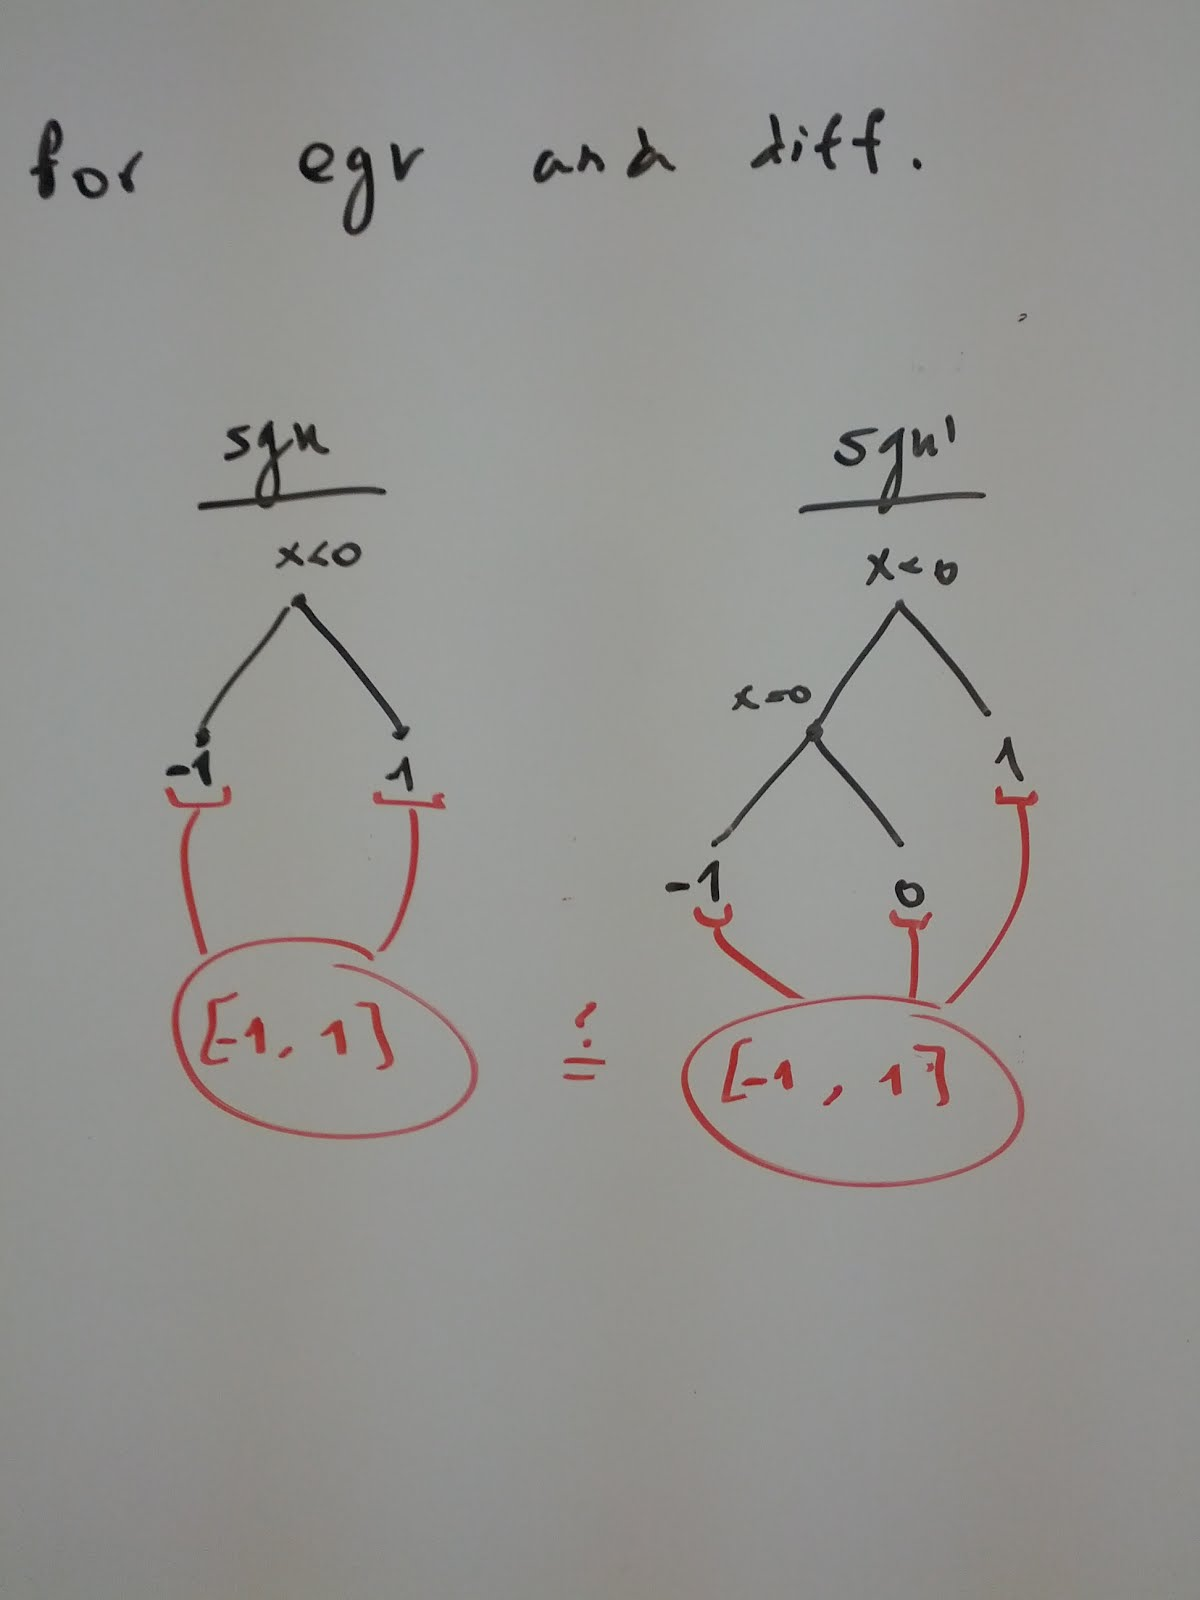
\includegraphics[scale=0.15,clip=true,trim = 125pt 400pt 125pt 350pt]{figures/sign-interval.jpg}
}
\caption{Interval analysis unsound comparison for $sign$ and $sign'$}\figlabel{SignInterval}
\end{wrapfigure}
Furthermore, this result entirely ignores how $x$ affects the value of $sgn$ thus we would have no means to differentiate equivalent inputs from offending ones (e.g. we will get the same result for the $-1 * sign$ function).

To establish equivalence under abstraction, we need to abstract relationships between the values of variables in $sign$ and $sign'$ under the assumption of equivalence of input. Specifically, we need to track the relationship between the values of \scode{sgn} in both versions and see whether we can establish their equivalence. Tracking relationships dictates performing a \emph{joint analysis} that employs a \emph{correlating abstraction} that will allow us to bind variables of both programs in one abstract state.

A correlating-oriented abstraction is well suited for proving equivalence as it allows focusing on relationships between versions of variables while abstracting away other (numerical) information allowing us to scale better. Most importantly, such an abstraction guarantees that equivalence will be reported soundly: as in a separate analysis we abstracted $\langle sgn \mapsto -1 \rangle$ and $\langle sgn \mapsto 1 \rangle$ towards an interval $\langle sgn \mapsto [-1,1] \rangle$, and again for $sgn'$ values, separately, which cannot assure equivalence, we will now abstract $\langle sgn = sgn' \mapsto -1 \rangle$ and $\langle sgn = sgn' \mapsto 1 \rangle$ as $\langle sgn = sgn' \rangle$ which soundly assures equivalence although all other variables information has been abstracted away.

%If we instead use disjunctive completion powerset domain~\cite{TODO} where the abstract state is a set of convex sub-states, and no merge is ever performed, this would yield a precise result that may be used for equivalence checking and differencing.  For instance, using such domain for $sign$ would yield: $\langle x < 0, sgn = -1 \rangle \vee \langle x \geq 0, sgn = 1 \rangle$ and for $sign'$: $\langle x < 0, sgn = -1 \rangle \vee \langle x > 0, sgn = 1 \rangle \vee \langle x = 0, sgn = 0 \rangle$. Further refining $sign$'s abstraction and splitting the $\langle x \geq 0, sgn = 1 \rangle$ constraint to $\langle x > 0, sgn = 1 \rangle \vee \langle x = 0, sgn = 0 \rangle$ would allow perfectly aligning the input constraints to produce the difference of $x=0,sgn=1,sgn'=0$ as depicted in \figref{SignComplete}.
%\begin{wrapfigure}{r}{0cm}
%\imagetop{
%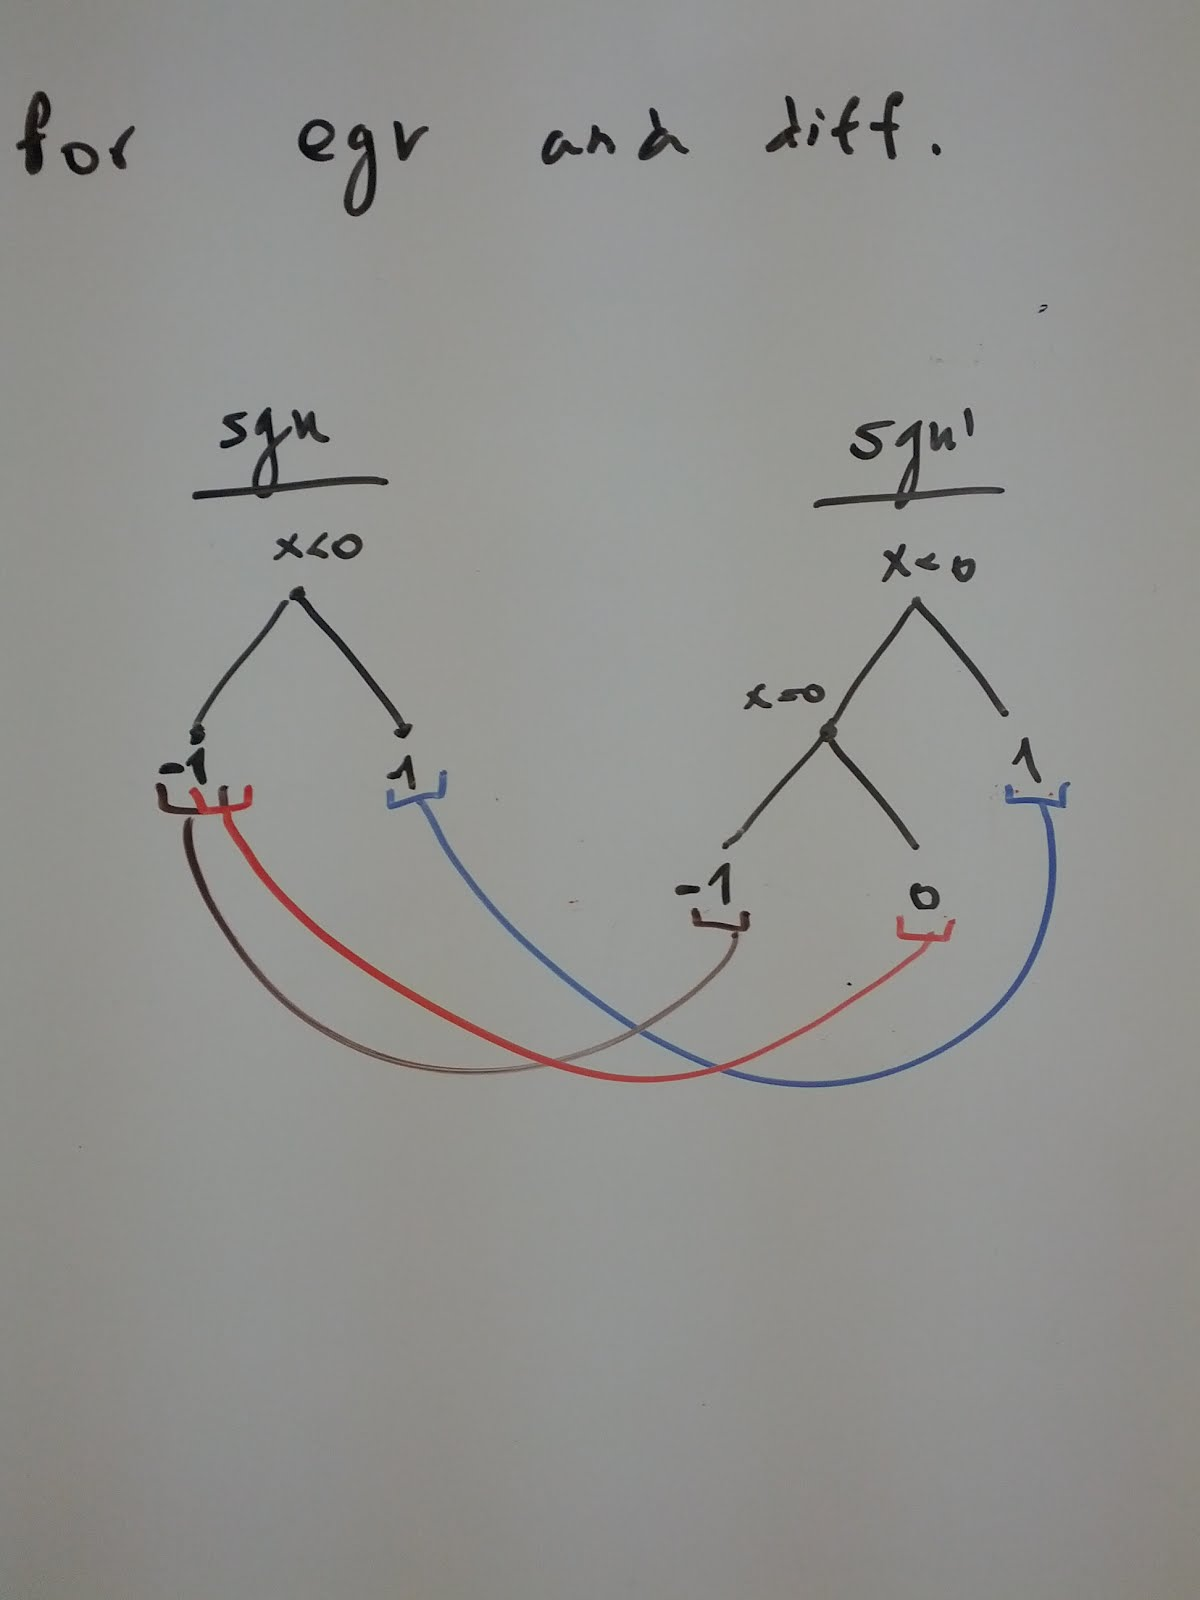
\includegraphics[scale=0.15,clip=true,trim = 125pt 450pt 100pt 350pt]{figures/sign-complete.jpg}
%}
%\caption{Complete disjunction analysis sound comparison for $sign$ and $sign'$}\figlabel{SignComplete}
%\end{wrapfigure}

We present an abstraction over dual program state, thats able to correlate paths that originate from the same input as well as produce a characterization of equivalence and difference which reflects change in behavior precisely. For example, we produce the following constraints for $sign$ and $sign'$:
\\
\begin{tabular}{ccc}
$x < 0$: & sgn = -1 & sgn' = -1
\\
$x = 0$: & sgn = 1 & sgn' = 0
\\
$x > 0$: & sgn = 1 & sgn' = 1
\\
\end{tabular}
\\
These constraints are a precise abstract description of equivalence and difference in $sign$ and $sign'$ and we will describe how we arrive at this result.

Initially, we abstracted the dual program state by analyzing both programs, sequentially, and updating the shared state with data regarding both sets of variables. We allow direct relationships between versions of variables, this will be of upmost importance later on when we over approximate paths for scalability. In order to correlate paths by input and arrive at a precise disjunction (\figref{SignResult}), we initially assume input equivalence $\vec{i} = \vec{i'}$. As we advance through the analysis of $P$, we will accumulate the disjunction of all possible path constraints in its final state (this is similar to trace partitioning~\cite{}). At this point, as we continue to analyze $P'$, each disjunct representing a path in $P$ will be further refined and conjunct with all of $P'$ paths. This will produce a precise disjunction for differencing as each path in $P$ will be split and conjuncted with all of $P'$ paths, while avoiding considering conjunctions that disagree on input due to our input equivalence assumption. An illustration of the joint analysis for the $sign$ example can be seen in \figref{SignAnalysis1} including markings for feasible and infeasible paths.

%In some cases, it would have been sufficient to use alternative domains that are capable of representing richer information, such as interval polyhedra~\cite{CMWC:SAS09}, or other numerical domains that can represent non-convex information (e.g., \cite{TODO}). The recent donut domain~\cite{GIBMG:VMCAI12} may be of particular interest for this purpose. However, the general principle of having to preserve correlating information even when information about the values is abstracted away, holds in all of these cases.

\begin{figure}
\imagetop{
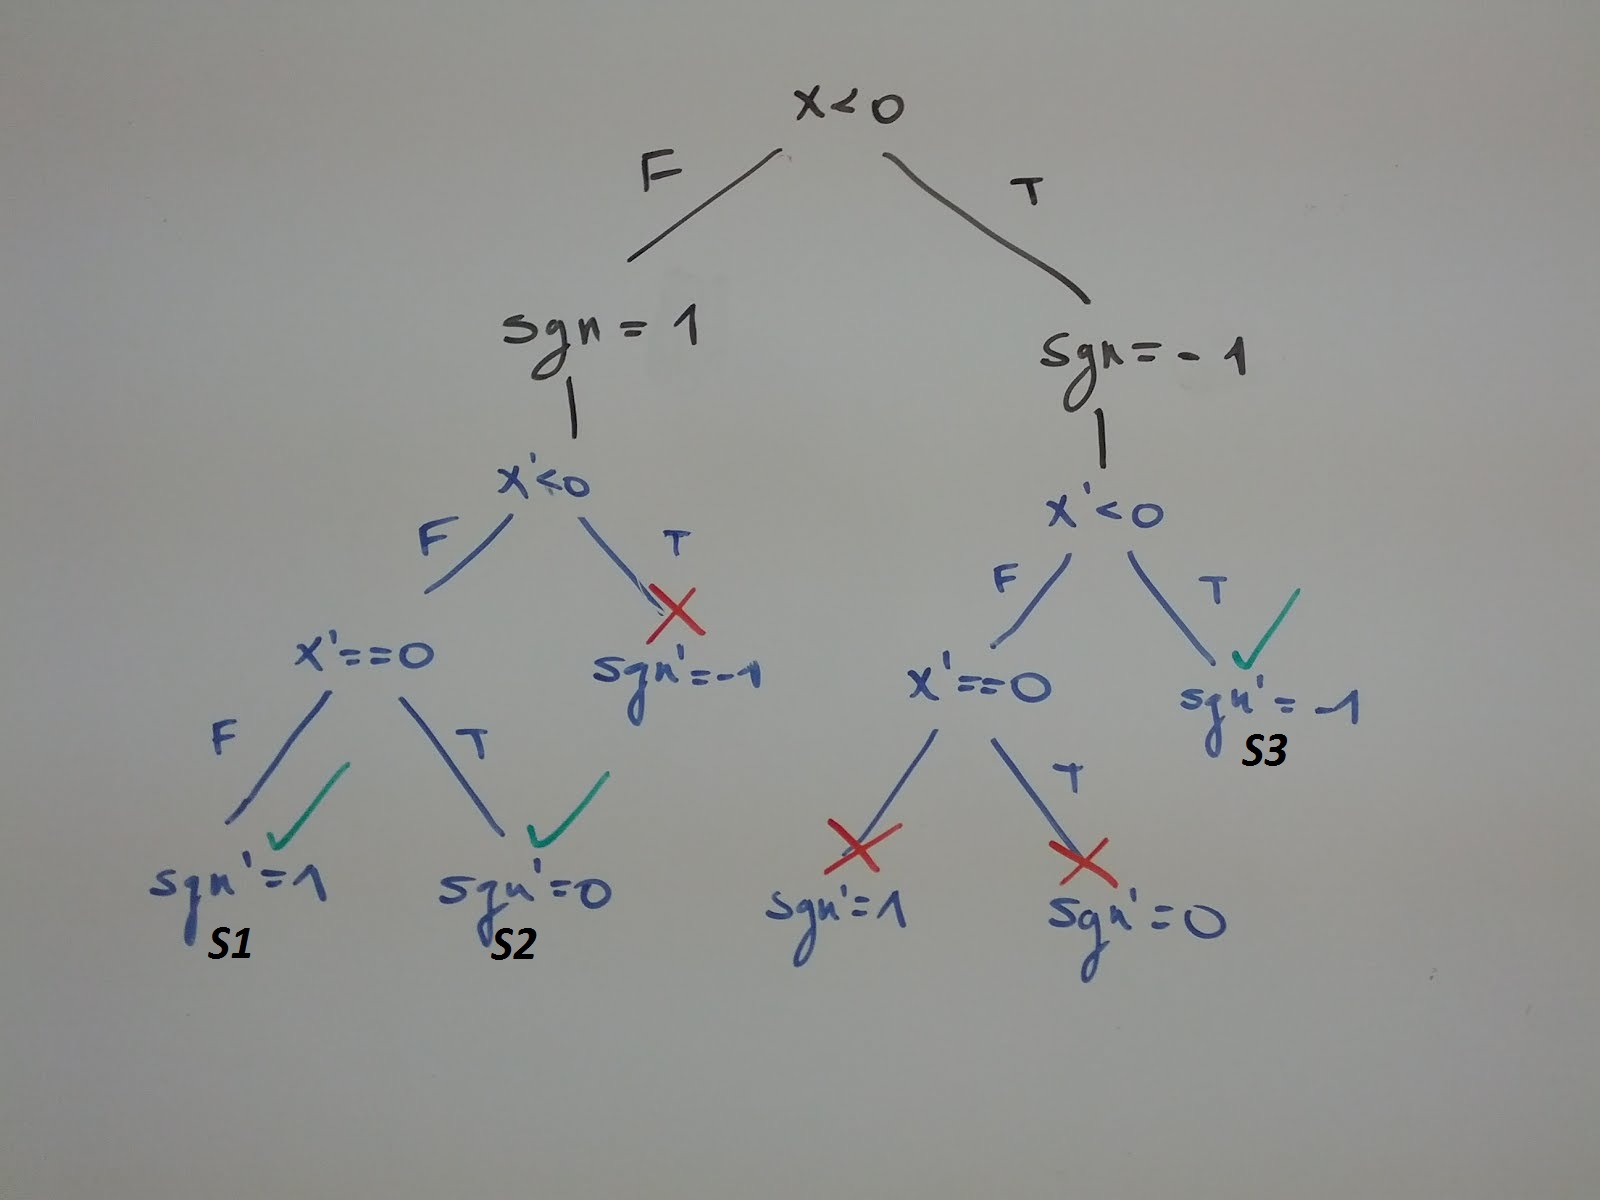
\includegraphics[scale=0.28,clip=true,trim = 50pt 100pt 100pt 0pt]{figures/sign-analysis1.jpg}
}
\caption{Joint $sign;sign'$ analysis}\figlabel{SignAnalysis1}
\end{figure}
Essentially, our analysis aims to establish correspondence between paths in $P$ and $P'$ by first analyzing all of $P$ paths and then attempting to correlate with $P'$ path. Analyzing over $P;P'$ means in the worst case remembering the states along each $P$-path and relating them to states in the corresponding $P'$-path. This approach is similar to the symbolic execution approach~\cite{} where all possible correlating paths are explored individually and output is examined to determine difference whilst attempting to reach full coverage. Much like this approach, this abstraction is unfeasible for most cases, especially for programs with an unbound number of paths e.g. \textbf{loops}. To avoid this we move to a partially disjunctive domain, partitioned by \emph{equivalence criteria}.

As the goal of work is to distinguish equivalent from differencing behaviors, using equivalence as criteria for merging paths is apt. The partitioning will abstract together paths that hold equivalence for the same set of variables, allowing for a maximum of $2^{|V|}$ disjunctions in the abstract state, where $V$ is the set of correlated (output?) variables. This criteria can be refined, by adding to $V$, to provide a more precise result or alternatively can become more coarse by allowing only certain equivalence classes of $2^{V}$.

For example partitioning the result of \figref{SignAnalysis1} according to our criteria would abstract behaviors $S1$ and $S3$ together, as they hold equivalence for $sgn$. The merge would abstract away data regarding $x$ and represent $sgn$ as the $[-1,1]$ interval, losing precision but gaining reduction in state size. This lose of precision is acceptable as it is complemented by the offending state $S2$. Still, not much is gained from this partitioning, as it is performed at the final state, where we may have already reached an exponential amount of disjunctions.
\begin{wrapfigure}{r}{0cm}
\imagetop{
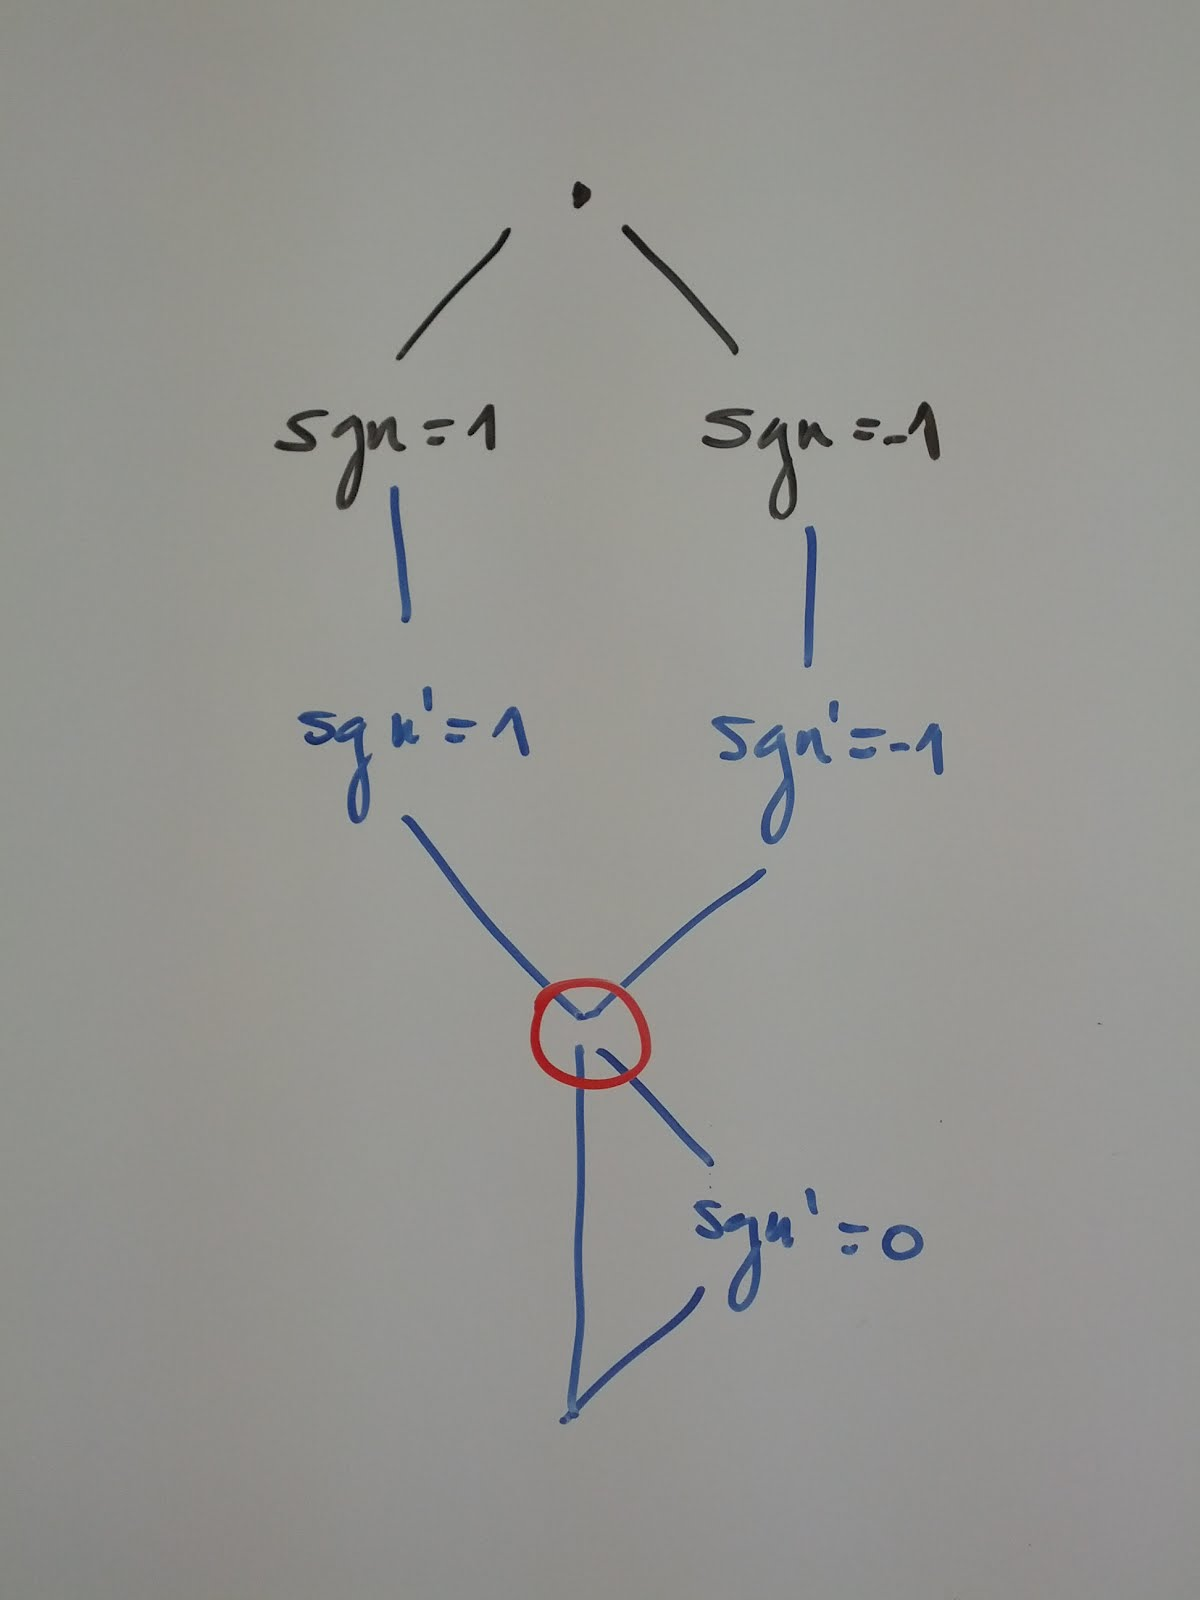
\includegraphics[scale=0.12,clip=true,trim = 250pt 150pt 200pt 150pt]{figures/sign-analysis2.jpg}
}
\caption{$sign \bowtie sign'$ analysis}\figlabel{SignAnalysis2}
\end{wrapfigure}
To truly gain a reduction of state size, we must perform partitioning dynamically, as the analysis is executed i.e. at earlier program locations. This cannot be achieved using a sequential composition $P;P'$. Looking at \figref{SignAnalysis1} we immediately see that equivalence holds only at final states. Intuitively, this is caused due to a command in one program having to "wait" for it's equivalent command to arrive from the second program. To overcome this, we present the correlating program denoted $P \bowtie P'$ which allows for earlier partitioning by "saving the need to wait" as it interleaves $P$ and $P'$ commands in an optimized manner, and informs the analysis that it need not wait any further and partitioning is permitted. \figref{SignAnalysis2} depicts the analysis of $sign \bowtie sign'$ (shown in \figref{SignCorrelating}) where the partitioning location is marked in red. We will further describe the specifics of creating $P \bowtie P'$ in \secref{Correlating} and only shortly say that the interleaving is chosen according to a syntactic diff process over a guarded command language version of the programs.

\begin{figure}
\centering
\begin{lstlisting}
// Nimrod - please fill this 
\end{lstlisting}
\caption{Correlating program $sign \correlate sign'$.}
\figlabel{SignCorrelating}
\end{figure}


% bite the bullet and do widening.
Although we achieved a reduction is state size using partitioning, we have yet to account for programs with an unbound number of paths, created by loops. Unbound path lengths means a potentially unbound analysis as all paths are abstracted. This is mainly where previous approaches fall short ~\cite{}. To overcome this, we define a widening operator for our domain, based on the convex sub-domain widening operator. The main challenge here, as our state is a set of convex objects, is finding an optimal pairwise matching between objects for a precise widened result. Optimally, we would like to pair objects that adhere to the same "looping path" meaning we would want to match $\pi_i$'s abstraction with a $\pi_{i+1}$ that results from taking another step in the loop. This basically requires encoding path information along with the sub-state abstraction. This information is acquired by simply keeping guard values explicitly, as they appear in our correlating program, inside the state. As guard values (true or false) reflect branch outcomes, they can be used to match sub-states that advanced on the loop by matching their guard values (for easier matching and better precision we separate guards from other variables in our implementation). \TODO{? simple loop example}.

\TODO{? maybe show a bigger example that better shows how we benefit from partitioning}

\TODO{? talk about how merging early in paths may affect equivalence and differencing behaviors further along}

\TODO{Say how the correlating program is crucial for the success of the analysis in the case of loops}

\TODO{also need to say that there is the problem of choosing differencing points} 